\section{Combinatorial Swap Landscape and Antipodal Traps}
\label{sec:landscape}

Whereas \Cref{sec:spectral} showed that the continuous quadratic form $\mathbf{z}^\top L_n \mathbf{z}$ on $\mathbf{1}^\perp$ is convex and barrier-free, restricting $\mathbf{z}$ to the discrete permutation polytope $S_{n^2}$ induces a rugged combinatorial energy landscape under elementary cell swaps. We now derive the exact algebraic law governing $2$-cycle transpositions and perform an exhaustive basin census of $S_9$ ($n=3$) and a large-scale relaxation census of $S_{16}$ ($n=4$).

\subsection{Exact Quadratic Transposition Law}

Let $\mathbf{g}(S) = \frac{1}{2}\nabla \Hline(\mathbf{z}) = L_n \mathbf{z} = A_n^\top \mathbf{R}(S) \in \Z^{n^2}$ denote the \emph{cell-stress vector}, whose component $g_a(S) = \sum_{L\ni a} R_L(S)$ at cell $a \in \{1,\dots,n^2\}$ is the sum of the centred residuals of the $2$, $3$, or $4$ magic lines passing through cell $a$. Swapping the values at cells $a$ and $b$ via the transposition $\tau_{ab} \in S_{n^2}$ replaces $\mathbf{z}$ by $\mathbf{z}' = \mathbf{z} - d(\mathbf{e}_a - \mathbf{e}_b)$, where $d = Z_a - Z_b = 2(s_a - s_b)$. Expanding $\mathbf{z}'^\top L_n \mathbf{z}'$ yields:

\begin{proposition}[Exact Transposition Energy Formula]
\label{prop:swap_law}
For any permutation $S \in S_{n^2}$ and any pair of cells $a \ne b$ with height difference $d = Z_a - Z_b$, the change in the line-indicator Hamiltonian under the transposition $\tau_{ab}$ is
\begin{equation}
  \Delta\Hline(\tau_{ab}) = \Hline(\tau_{ab} S) - \Hline(S) = -2d\bigl(g_a(S) - g_b(S)\bigr) + c_{ab}\,d^2,
  \label{eq:exact_swap_delta}
\end{equation}
where $c_{ab} = (L_n)_{aa} + (L_n)_{bb} - 2(L_n)_{ab} = \|A_n(\mathbf{e}_a - \mathbf{e}_b)\|_2^2 \in \{2,3,4,5,6,7,8\}$ counts the number of magic lines in $\mathcal{L}_n$ that pass through \emph{exactly one} of the two cells $a$ and $b$. In particular, $\Delta\Hline(\tau_{ab}) < 0$ if and only if $(g_a - g_b)/d > c_{ab}/2$.
\end{proposition}

\Cref{prop:swap_law} explains why discrete $2$-cycle descent becomes frustrated near the ground state: when line residuals $R_L(S)$ are small ($\pm 2$ in centred units, or $\pm 1$ in standard units), the linear stress release $-2d(g_a - g_b)$ has magnitude $O(|d|)$, whereas the quadratic self-energy penalty $c_{ab}d^2 \ge 8$ (since $|d| \ge 2$ and $c_{ab} \ge 2$) grows quadratically with the height jump $|d|$ and blocks any single transposition from lowering $\Hline$.

\begin{figure}[t]
  \centering
  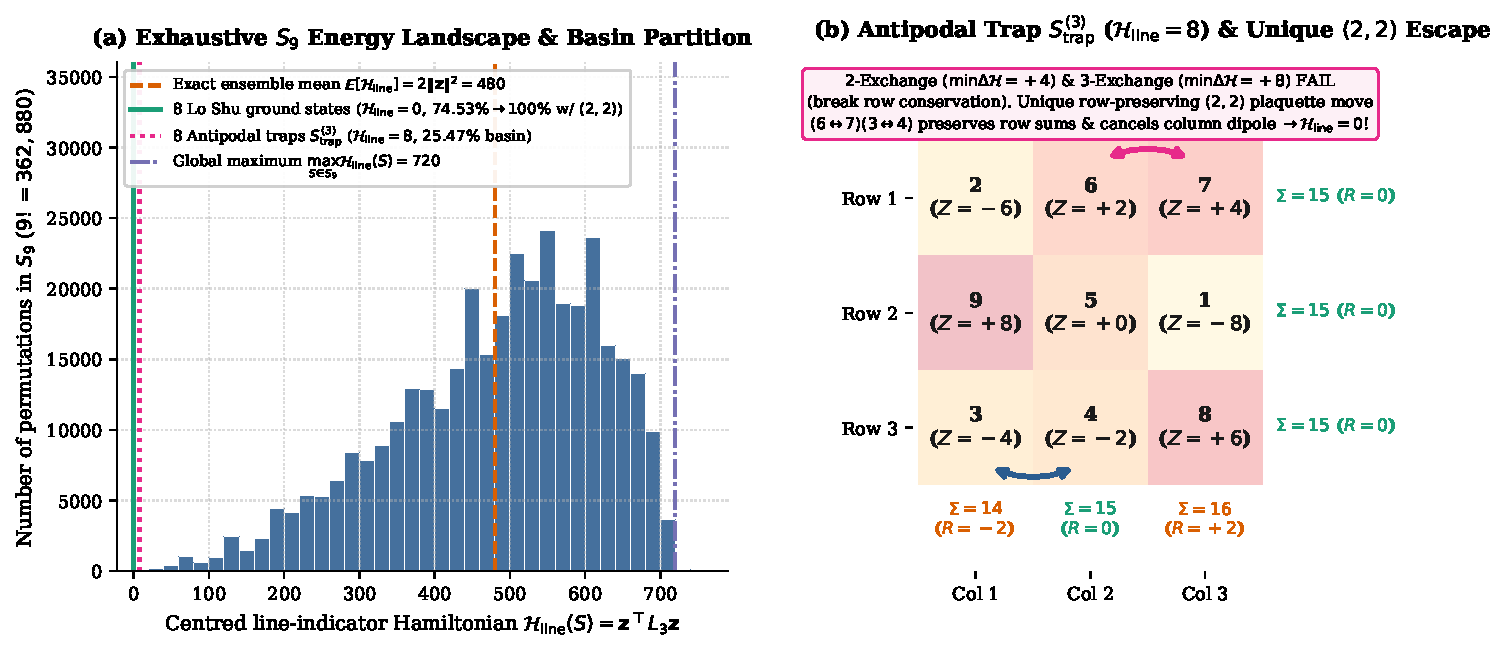
\includegraphics[width=\textwidth]{figures/fig4_s9_landscape_traps.pdf}
  \caption{\textbf{Exhaustive $S_9$ permutation landscape ($362{,}880$ states) and the $8$ antipodal traps at order $n=3$.} \textbf{(a)} Exact histogram of the centred line Hamiltonian $\Hline(S)$ across all $9! = 362{,}880$ states of $S_9$, showing the ensemble mean $\mathbb{E}[\Hline]=480$ (\Cref{thm:ensemble_mean}), the $8$ Lo Shu ground states at $\Hline=0$, and the $8$ strict local-minimum traps $S_{\mathrm{trap}}^{(3)}$ at $\Hline=8$. \textbf{(b)} Structure of the canonical trap $S_{\mathrm{trap}}^{(3)}$ (\Cref{thm:s9_traps}): all $3$ rows, the middle column, and both main diagonals sum to $15$ ($R=0$), while the outer columns sum to $14$ ($R=-2$) and $16$ ($R=+2$). Every $2$-cycle ($\min\Delta\Hline = +4$) and every $3$-cycle ($\min\Delta\Hline = +8$) strictly increases energy; escaping to the Lo Shu ground state requires the simultaneous $(2,2)$ double swap $(2\leftrightarrow 4)(3\leftrightarrow 1)$.}
  \label{fig:s9_landscape}
\end{figure}

\subsection{Exhaustive \texorpdfstring{$S_9$}{S9} Landscape Census and the 8 Antipodal Traps of Order 3}

At order $n=3$, the symmetric group $S_9$ has $9! = 362{,}880$ states, permitting an exact, exhaustive classification of the entire combinatorial energy landscape (\Cref{thm:s9_traps} and \Cref{fig:s9_landscape}):

\begin{theorem}[Exhaustive $S_9$ Landscape and the $8$ Strict Local Minima of Order 3]
\label{thm:s9_traps}
Across all $9! = 362{,}880$ permutations of $S_9$ under the line-indicator Hamiltonian $\Hline(S)$:
\begin{enumerate}
  \item \textbf{Complete Classification of Local Minima:} There are \textbf{exactly $16$ local minima} in $S_9$ under the $\binom{9}{2} = 36$ elementary $2$-cycle transpositions, all $16$ of which are strict local minima ($\Delta\Hline(\tau_{ab}) > 0$ for all $a \ne b$):
  \begin{itemize}
    \item The \textbf{$8$ global ground states} ($\Hline = 0$), forming the single dihedral orbit $D_4 \cdot S_{\mathrm{LoShu}}$.
    \item \textbf{Exactly $8$ spurious strict local minima} at $\Hline = 8$ ($E_{\mathrm{std}} = 2$), forming the single dihedral $D_4$ orbit of the antipodal trap
    \begin{equation}
      S_{\mathrm{trap}}^{(3)} = \begin{bmatrix}
        2 & 6 & 7 \\
        9 & 5 & 1 \\
        3 & 4 & 8
      \end{bmatrix}, \qquad
      \mathbf{Z}\bigl(S_{\mathrm{trap}}^{(3)}\bigr) = \begin{bmatrix}
        -6 & +2 & +4 \\
        +8 & 0 & -8 \\
        -4 & -2 & +6
      \end{bmatrix}, \qquad \Hline\bigl(S_{\mathrm{trap}}^{(3)}\bigr) = 8.
      \label{eq:S_trap_3}
    \end{equation}
  \end{itemize}
  \item \textbf{Instability Under $2$-Cycles and $3$-Cycles, and $(2,2)$-Cycle Escape:} In $S_{\mathrm{trap}}^{(3)}$, six of the eight magic lines (all three rows, the middle column, and both main diagonals) have zero residual ($R_L = 0$), while the two outer columns have residuals $R_{c_1} = -2$ ($\Sigma=14$) and $R_{c_3} = +2$ ($\Sigma=16$). Every single $2$-cycle transposition strictly increases $\Hline$ by at least $+4$ ($\min_{\tau_{ab}} \Delta\Hline = +4$), \textbf{and every single $3$-cycle permutation among all $2\binom{9}{3} = 168$ directed $3$-cycles also strictly increases $\Hline$ by at least $+8$}. Escaping $S_{\mathrm{trap}}^{(3)}$ to the Lo Shu ground state requires a simultaneous disjoint double transposition ($(2,2)$-cycle), such as $(2\leftrightarrow 4)(3\leftrightarrow 1)$ or $(6\leftrightarrow 4)(7\leftrightarrow 9)$.
  \item \textbf{Exact Steepest-Descent Basin Partition:} Under deterministic $2$-cycle steepest descent (choosing the lexicographically first pair $(a,b)$ minimizing $\Delta\Hline(\tau_{ab})$), \textbf{$270{,}442$ of the $362{,}880$ states ($74.5266\%$) converge to the $8$ Lo Shu ground states}, while the remaining \textbf{$92{,}438$ states ($25.4734\%$) are captured by the $8$ antipodal traps $D_4 \cdot S_{\mathrm{trap}}^{(3)}$}.
\end{enumerate}
\end{theorem}

\begin{proof}
All $362{,}880$ permutations of $S_9$, their $36$ transposition deltas $\Delta\Hline(\tau_{ab})$ via \Cref{eq:exact_swap_delta}, all $168$ directed $3$-cycle deltas on trapped states, and the steepest-descent attractor map are evaluated exhaustively in \texttt{verify\_paper\_d.py} (\Cref{fig:s9_landscape}). To see algebraically why $S_{\mathrm{trap}}^{(3)}$ in \Cref{eq:S_trap_3} is immune to both $2$-cycles and $3$-cycles: in standard units $s_{ij} - 5 \in \{-4,\dots,4\}$, $E_{\mathrm{std}}(S_{\mathrm{trap}}^{(3)}) = (-1)^2 + (+1)^2 = 2$. Reducing $E_{\mathrm{std}}$ below $2$ requires reaching a state where at most one line has residual $\pm 1$ (impossible by parity) or reaching $E_{\mathrm{std}} = 0$ directly. Because every row sum of $S_{\mathrm{trap}}^{(3)}$ is already $15$, any single $2$-cycle between different rows alters two row sums by $\pm d \ne 0$ (adding $2d^2 \ge 2$ to the row energy), while any within-row $2$-cycle changes the diagonal sums by at least $\pm 2$. Similarly, any $3$-cycle either touches two cells in one row and one cell in another row (breaking both row sums) or touches one cell in each of the three rows (preserving row sums only if all three swapped values are identical, which is impossible). By contrast, a simultaneous disjoint $(2,2)$ double transposition such as $(2\leftrightarrow 4)(3\leftrightarrow 1)$ exchanges $(-1)$ and $(+1)$ across two rows simultaneously, lowering $E_{\mathrm{std}}$ and unlocking direct descent to the Lo Shu ground state.
\end{proof}

\subsection{Order-4 (\texorpdfstring{$S_{16}$}{S16}) Steepest-Descent Basin Census}

At order $n=4$, the state space $S_{16}$ grows to $16! \approx 2.09 \times 10^{13}$ permutations, while the number of distinct magic ground states is $880 \times 8 = 7{,}040$. To quantify local-minimum trapping in $S_{16}$, we performed $2{,}000$ independent steepest-descent trials starting from uniform random permutations (\Cref{fig:s16_descent} and \Cref{tab:s9_s16_landscape}).

\begin{figure}[t]
  \centering
  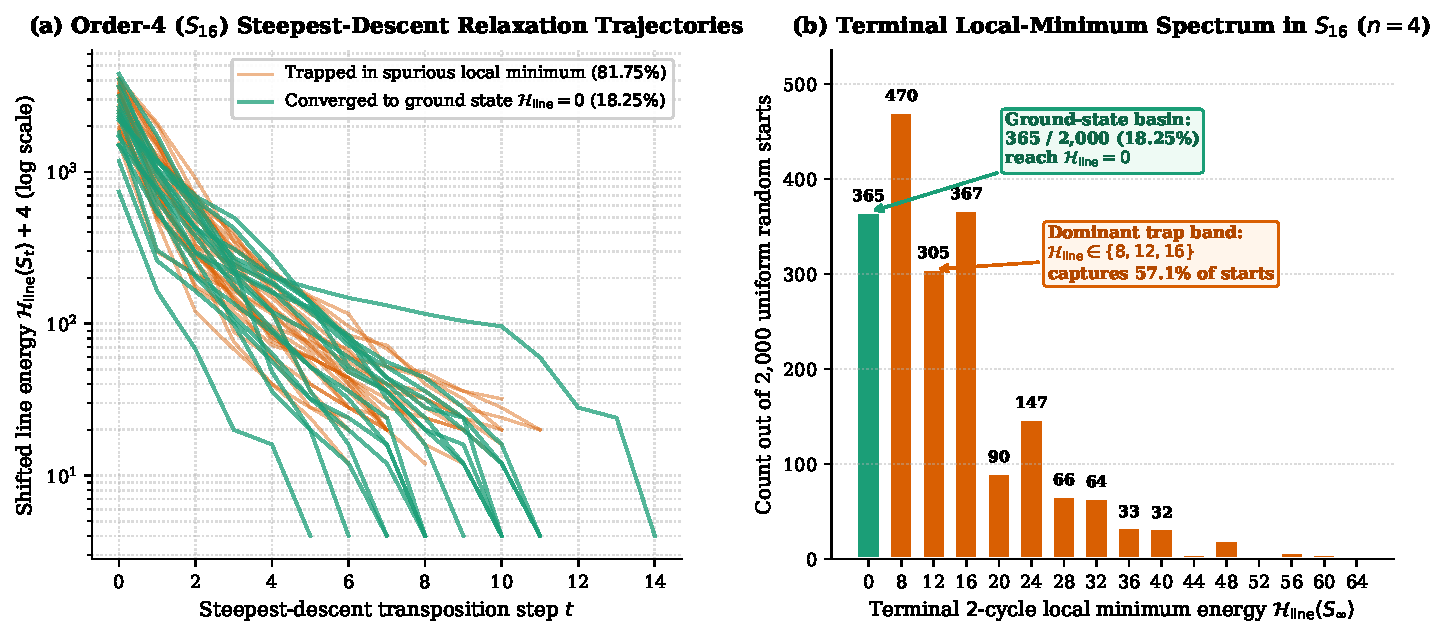
\includegraphics[width=\textwidth]{figures/fig5_s16_descent_basins.pdf}
  \caption{\textbf{Order-$4$ ($S_{16}$) steepest-descent relaxation trajectories and local-minimum spectrum ($2{,}000$ trials).} \textbf{(a)} Representative steepest-descent trajectories of $\Hline(S_t) + 4$ (log scale) versus transposition step $t$, contrasting trajectories that reach the magic ground state $\Hline=0$ (green, $18.25\%$) against trajectories trapped in frustrated local minima (orange, $81.75\%$). \textbf{(b)} Histogram of terminal $2$-cycle local-minimum energies $\Hline(S_\infty)$ across $2{,}000$ uniform random starts in $S_{16}$. While $365/2{,}000$ ($18.25\%$) reach $\Hline=0$, $57.1\%$ of all starts become trapped in the low-energy frustration band $\Hline \in \{8,12,16\}$.}
  \label{fig:s16_descent}
\end{figure}

As shown in \Cref{fig:s16_descent}b and \Cref{tab:s9_s16_landscape}, pure $2$-cycle steepest descent in $S_{16}$ reaches a magic ground state ($\Hline = 0$) in only $365 / 2{,}000$ trials ($18.25\%$), terminating in a mean of $8.18$ steps at a mean residual energy $\langle\Hline(S_\infty)\rangle = 14.43$ (median $12.0$). The trapped configurations cluster heavily in the lowest frustration band $\Hline \in \{8, 12, 16\}$, which accounts for $470 + 305 + 367 = 1{,}142 / 2{,}000$ ($57.1\%$) of all random starts. Testing all $2\binom{16}{3} = 1{,}120$ directed $3$-cycles on each of the $1{,}635$ trapped $2$-cycle local minima reveals that $56$ ($3.43\%$) immediately escape via a single $3$-cycle, motivating the hybrid continuous-discrete solver developed in \Cref{sec:bubble}.

\begin{table}[t]
\centering
\caption{Summary of combinatorial swap-landscape invariants for $S_9$ ($n=3$, exhaustive $362{,}880$ states) and $S_{16}$ ($n=4$, $2{,}000$ random starts), verified by \texttt{verify\_paper\_d.py}.}
\label{tab:s9_s16_landscape}
\footnotesize
\setlength{\tabcolsep}{4pt}
\begin{tabular}{@{}lcc@{}}
\toprule
Landscape Observable / Metric & Order $n=3$ ($S_9$, Exhaustive) & Order $n=4$ ($S_{16}$, $2{,}000$ Trials) \\
\midrule
Total permutation state space $n^2!$ & $362{,}880$ & $20{,}922{,}789{,}888{,}000$ \\
Magic ground states ($\Hline = 0$) & $8$ ($1\times D_4$ orbit) & $7{,}040$ ($880\times D_4$ orbits) \\
Ensemble mean energy $\mathbb{E}[\Hline(S)] = 2\|\mathbf{z}\|^2$ & $480$ & $2{,}720$ \\
Elementary $2$-cycle neighborhood size $\binom{n^2}{2}$ & $36$ & $120$ \\
Directed $3$-cycle neighborhood size $2\binom{n^2}{3}$ & $168$ & $1{,}120$ \\
Spurious $2$-cycle local minima ($\Hline > 0$) & Exactly $8$ (at $\Hline=8$) & Abundant ($\Hline \in \{8,12,16,\dots\}$) \\
$2$-cycle steepest-descent ground-state basin & $270{,}442 / 362{,}880$ ($74.53\%$) & $365 / 2{,}000$ ($18.25\%$) \\
Mean terminal $\Hline(S_\infty)$ under $2$-cycle descent & $2.04$ & $14.43$ (median $12.0$) \\
\bottomrule
\end{tabular}
\end{table}
